\section{Dimensionality Reduction}
\subsection{The Curse of Dimensionality}
One of the characteristic of high-dimensional data is that the number of dimensions is comparable or larger than the number of samples.
High dimensional data is very sparse
\begin{table}[!h]
    \begin{tabular}{l|l}
        \hline
     Dim \(d\)& \(n\) for 10\% coverage \\
     \hline
     1&  10\\
     2&  100\\
     3&  1000\\
     10& \(10^10\)\\
     d& \(10^d\)
    \end{tabular}
    \end{table}
\subsection{The Manifold Hypothesis}
A collection of methodologies for analyzing high dimensional data based on the hypothesis that data tend to lie near a low dimensional manifold is now called Mainfold learning.
\subsection{Principal Component Analysis (PCA)}
The main linear technique for dimensionality reduction, mapping the data in such a way that the variance of the data in the low-dimensional representation is maximized.
\subsubsection{Eigenvalues \(\lambda_k\) of \(
C\) are the variance in the new space}
We are given \(i = 1 \dots n\) samples of dimension\((1 \times d)\)
We constuct the data matrix \(n\times d\): \(X_{ik} = \left[x_{ik}\right]\)

We diagonalize the covariance matrix \(C\):
\[
C = \frac{1}{n-1}(X-\overline{X})^T (X-\overline{X})
\]
if \(\overline{X} = 0\):
\[
C = \frac{1}{n-1}X^T X
\]
\[
C = UDU^T = U\left[\text{diag}(\lambda_k)\right]U^T
\]
\subsubsection{Explained variance}
No data is lost in transformation.
The first component explains most of the variance, the second the second most,\dots All components explain the whole variance.
Now take only a few components (the first \(k\)) and hope that the data is explained by them.
How good is the approximation?
A measure is the \textbf{explained variance ratio}:
\[
P_k = \frac{\sum_{j = 1}^k\textbf{VAR}(Z:,j)}{\sum_{j = 1}^d\textbf{VAR}(Z:,j)} = \frac{\sum_{j = 1}^k\lambda_j}{\sum_{j = 1}^d\lambda_j} 
\]
\subsubsection{Eigenvalue problem}
\[
\mathbf{CW}-\lambda\mathbf{w} = 0
\]
\[
(\mathbf{C}-\lambda\cdot\mathbf{I})\mathbf{w} = 0
\]
\[
\det(\mathbf{C}-\lambda\mathbf{I}) = 0
\]
\subsection{Mainfold Methods based on similarity}
\subsubsection{Example of metrics}
\(L_p\) metric: \(d_p(x,y) = ||x-y||_p = \sqrt[p]{\sum_i|x_i-y_i|^p}\)

\(L_\infty\) metric: \(||x||_\infty = \max_i\left\{|x_i|\right\}\)

\(L_1\) metric: \(d_1(x,y) = ||x-y||_1 = \sum_i|x_i-y_i\) (manhatten distance)

\subsubsection{MDS: Multidimensional scaling}
MDS attemps to model similarity or dissimilarity data as distance in geometric spaces.
In general, is a technique used for analyzing similarity or dissimilarity data.
MDS attemps to find an embedding from the high dimensional objects in \(I\) into \(y_i \in \mathbb{R}^d\) such that distances \(d_{ij}\) are preserved.
\subsubsection{LLE: local linear embedding}
LLE discribes the local properties of the manifold around a data point \(x_i\) by writing the data point as a linear combination (the so-called reconstruction weights \(w_{ij}\)) of its \(k\) nearest neighbor:
\[
x_i \approx \sum_{j = 1}^k w_{ij}x_j
\]
In the low dimension, LLE attemps to retain the reconstruction weights \(W\) as well as possible. Hence, LLE fits a hyperplane through the data point \(x_i\) and its nearest neighbors, thereby assuming that the mainfold is locally linear.
Finding the low \(d\)-dimensional data representation \(Y\) amounts to minimizing the cost function \(\mathcal{L}\):
\[
\mathcal{L}(w,Y) = \sum_{i = 1}^{N}||y_i - \sum_{j = 1}^{k}w_{ij}y_j||^2
\]
\begin{figure}[!h]
    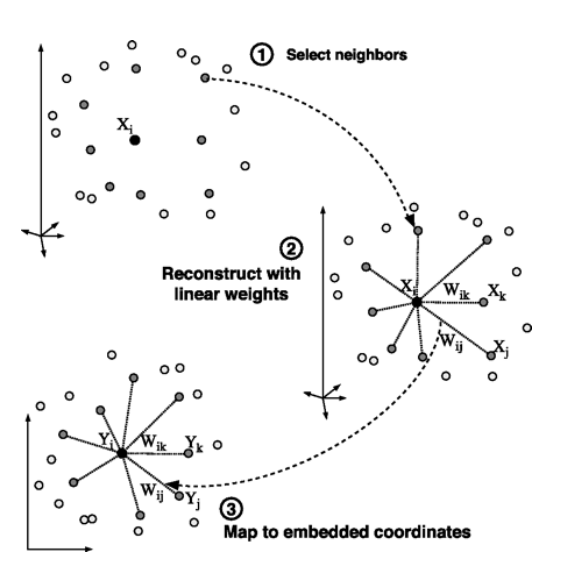
\includegraphics[width = \columnwidth]{figures/10/LLE.png}
\end{figure}
\subsubsection{Isomap: Isometric mapping}
\subsubsection{t-SNE:t-distributed stochastic neighbor embedding}